\documentclass[11pt,a4paper]{amsart}

\usepackage[english]{babel}
\usepackage[T1]{fontenc}
%\usepackage[latin1]{inputenc}
\usepackage{graphicx}
\usepackage[headings]{fullpage}

\makeatletter
\newcommand{\ps@bw}{%
  \renewcommand{\@oddhead}{%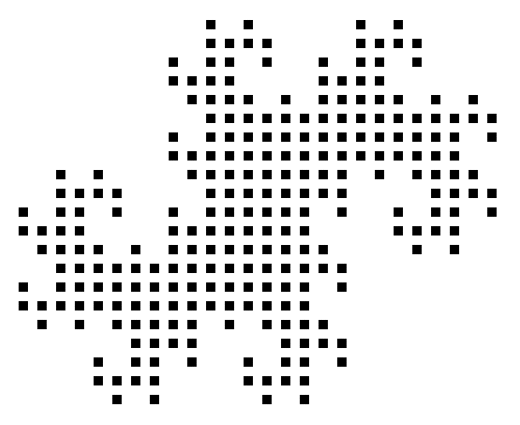
\includegraphics[height=2cm]{logo.png}\hfill English
\parbox[c]{5cm}{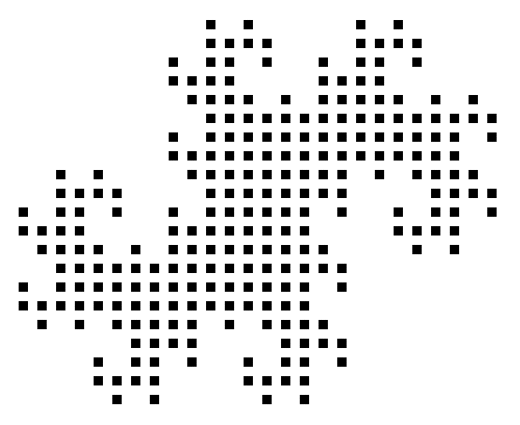
\includegraphics[height=2cm]{logo.png}}
 \hfill \parbox[b]{6cm}{\scshape\small\flushright English}
}%
  \renewcommand{\@evenhead}{}%
  \renewcommand{\@evenfoot}{}%
  \renewcommand{\@oddfoot}{}}
\makeatother

\theoremstyle{definition}
\newtheorem{prob}[section]{Problem}

\newcommand{\R}{\mathbb{R}}

\title{Baltic Way 2010}

\author[Baltic Way 2010]{Reykjavik, November 6th 2010}


\begin{document}

\maketitle
\thispagestyle{bw}

\noindent
Time allowed: $4\frac12$ hours.\\
Questions may be asked during the first 30 minutes.\\
The only tools allowed are a ruler and a compass.\\
Each problem is worth 5 points.\\




\maketitle

\prob
Find all quadruples of real numbers $(a,b,c,d)$ satisfying the system of equations
\[\begin{cases}
  (b+c+d)^{2010}=3a \\
  (a+c+d)^{2010}=3b \\
  (a+b+d)^{2010}=3c \\
  (a+b+c)^{2010}=3d.
\end{cases}\]



\prob
Let $x$ be a real number such that $0<x<\frac{\pi}{2}$. Prove that
\[
\cos^2 (x)\cot (x)+\sin^2 (x)\tan (x)\ge 1.\]


\prob
Let $x_1$, $x_2$, $\ldots$, $x_n$ ($n\geq 2$) be real numbers
greater than $1$. Suppose that $|x_i-x_{i+1}|<1$ for $i=1,2,\ldots,n-1$.
Prove that
$$\frac{x_1}{x_2}+\frac{x_2}{x_3}+\ldots+\frac{x_{n-1}}{x_n}+\frac{x_n}{x_1}<2n-1.$$


\prob
Find all polynomials $P(x)$ with real coefficients such that
\[(x-2010)P(x+67)=xP(x)\]
for every integer $x$.


\prob
Let $\R$ denote the set of real numbers. Find all functions $f:\R\rightarrow\R$ such that
\[f(x^2)+f(xy)=f(x)f(y)+yf(x)+xf(x+y)\]
for all $x,y\in\R.$


\prob
An $n\times n$ board is coloured in $n$ colours such that
the main diagonal (from top-left to bottom-right) is coloured in the first colour;
the two adjacent diagonals are coloured in the second colour; the two next diagonals
(one from above and one from below) are coloured in the third colour, etc.;
the two corners (top-right and bottom-left) are colored in the $n$-th colour.
It happens that it is possible to place on the board $n$ rooks, no two attacking each other and 
such that no two rooks stand on cells of the same colour.
Prove that $n\equiv 0\pmod{4}$ or $n\equiv 1\pmod{4}$.


\prob
There are some cities in a country; one of them is the capital.
For any two cities $A$ and $B$ there is a direct flight from $A$ to $B$ and a direct flight from $B$ to $A$, both having the same price.
Suppose that all round trips with exactly one landing in every city have the same total cost. Prove that all round trips that miss the capital and with exactly one landing in every remaining city cost the same.


\prob
In a club with $30$ members, every member initially had a hat.
One day each member sent his hat to a different member
(a member could have received more than one hat).
Prove that there exists a group of $10$ members such that
no one in  the group has received a hat from another
one in the group.


\prob
There is a pile of 1000 matches. Two players each take turns and can take up to 5 matches.
It is also allowed at most 10 times during the whole game to take 6 matches,
for example 7 exceptional move can be done by the first player and 3 moves by the second and then no more exceptional moves are allowed.
Whoever takes the last match wins.
Determine which player has a winning strategy.


\prob
Let $n$ be an integer with $n\geq 3$. 
Consider all dissections of a convex $n$-gon into triangles by 
$n-3$ non-intersecting diagonals, and all 
colourings of the triangles with black and white so that triangles with a 
common side are always of a different colour. Find the least possible number
of black triangles.

\prob
Let $ABCD$ be a square and let $S$ be the point of intersection of its diagonals $AC$ and $BD$. Two circles  $k$, $k'$ go through $A$, $C$ and $B$, $D$; respectively. Furthermore, $k$ and $k'$ intersect in exactly two different points $P$ and $Q$. Prove that $S$ lies on $PQ$.


\prob
Let $ABCD$ be a convex quadrilateral with precisely one pair of parallel sides.

\begin{itemize}
 \item[a)] Show that the lengths of its sides $AB$, $BC$, $CD$, $DA$ (in this order) do not form an arithmetic progression.
\item[b)] Show that there is such a quadrilateral for which 
the lengths of its sides $AB$, $BC$, $CD$, $DA$ form an arithmetic progression after the order of the lengths is changed. 
\end{itemize}


\prob
In an acute triangle $ABC$, the segment $CD$ is an altitude and $H$
is the orthocentre. Given that the circumcentre of the triangle lies
on the line containing the bisector of the angle $DHB$,
determine all possible values of $\angle CAB$.

\prob
Assume that all angles of a triangle $ABC$ are acute. 
Let $D$ and $E$ be points on the sides $AC$ and $BC$ of the triangle such that $A, B, D$, and $E$ lie on the same circle. Further suppose the circle through $D, E$, and $C$ intersects the side $AB$ in two points $X$ and $Y$. Show that the midpoint of $XY$ is the foot of the altitude from $C$ to $AB$.


\prob
The points $M$ and $N$ are chosen on the bisector $AL$ of a triangle $ABC$
such that  $\angle ABM=\angle ACN=23^\circ$.
$X$ is a point inside the triangle such that $BX=CX$ and $\angle BXC=2\angle BML$.
Find $\angle MXN$.

\prob
For a positive integer $k$, let $d(k)$ denote the number of divisors of $k$ (e.g.\ $d(12) = 6$) and let $s(k)$ denote the digit sum of $k$ (e.g.\ $s(12) = 3$). A positive integer $n$ is said to be {\em amusing} if there exists a positive integer $k$ such that $d(k) = s(k) = n$. What is the smallest amusing odd integer greater than 1? 


\prob
Find all positive integers $n$ such that the decimal representation of $n^2$
consists of odd digits only.

\prob
Let $p$ be a prime number.
For each $k$, $1\le k\le p-1$, there exists a unique integer denoted by $k^{-1}$ such that  $1\le k^{-1}\le p-1$ and
$k^{-1}\cdot k\equiv 1\pmod p$.
Prove that the sequence
\[
1^{-1}, \quad 1^{-1}+2^{-1},\quad 1^{-1}+2^{-1}+3^{-1}, \quad\dots, \quad 1^{-1}+2^{-1}+\dots+(p-1)^{-1}
\]
(addition modulo $p$) contains at most $(p+1)/2$ distinct elements.

\prob
For which $k$ do there exist $k$ pairwise distinct primes $p_1, p_2, \dots, p_k$ such that
\[p_1^2+p_2^2+\dots+p_k^2=2010 ?\]

\prob
Determine all positive integers $n$ for which there exists an infinite subset $A$ of the set $\mathbb N$ of positive integers such that for all pairwise distinct $a_1, \dots, a_n \in A$ the numbers $a_1 + \dots + a_n$ and $a_1\cdots a_n$ are coprime.


\end{document}
